\documentclass[a4paper, 11pt]{article}
\usepackage{geometry}
\usepackage{graphicx}
\usepackage{a4wide}
\usepackage{ulem}
\usepackage{amsthm}
\usepackage{amsmath}
\usepackage{amsfonts}
\usepackage{amssymb}
\usepackage[T1]{fontenc}
\usepackage{ngerman}
\usepackage{graphicx}
\usepackage{epic}
\usepackage{enumerate}
\usepackage{tabu}
\usepackage [latin1]{inputenc}
\geometry{a4paper,left=15mm,right=25mm,top=10mm,bottom=15mm}
%\renewcommand{\baselinestretch}{1.5}
\newcommand{\ol}{\overline}
\newcommand{\makeline}{\hrule\vspace{5pt}}
\newcommand{\ip}[2]{\left< #1, #2 \right>}

\title{6. �bungsblatt zu Software Qualit�t}
\author{Michel Meyer, Manuel Schwarz}

\begin{document}
  \maketitle

  \section*{Aufgabe 6.1}
  \subsection*{(a)}
  %\begin{figure}
		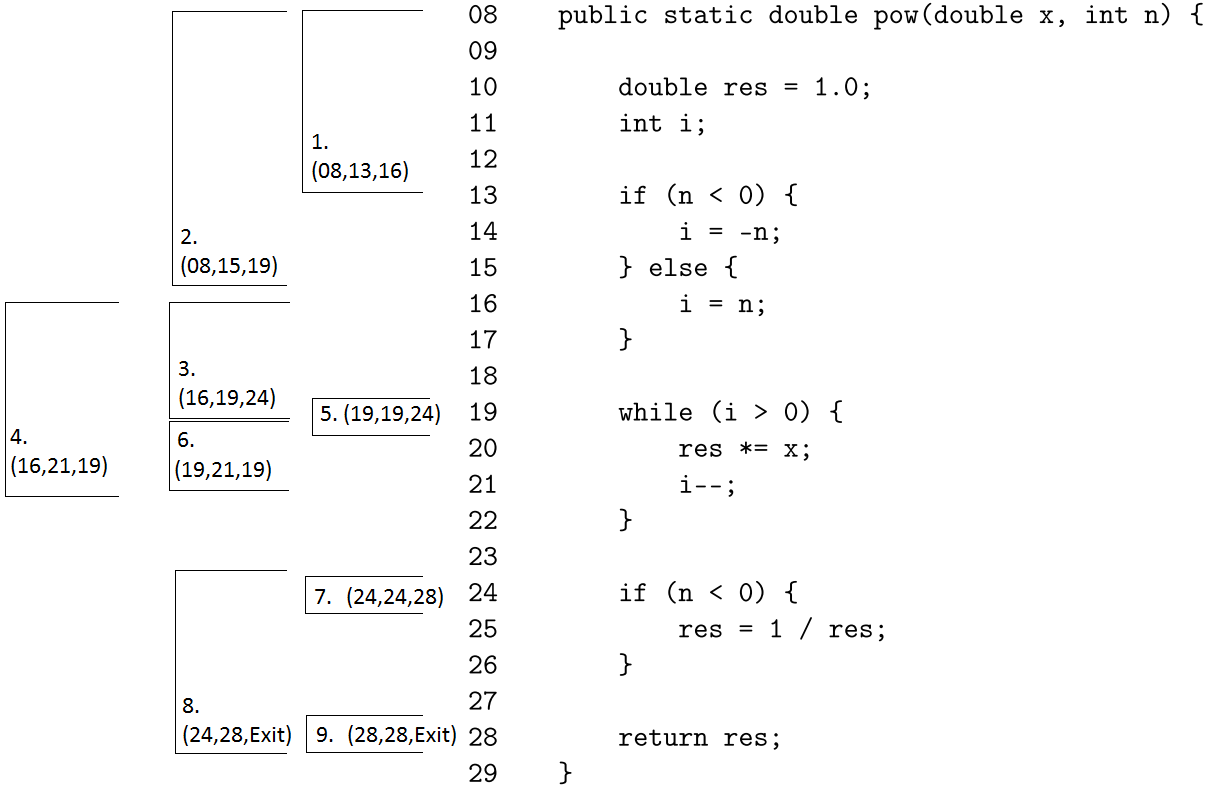
\includegraphics[width=\columnwidth]{Aufg6_1.png}
	%\end{figure}
  

  \section*{Aufgabe 6.2}

  \subsection*{(a) Kontrollflussgraph}
		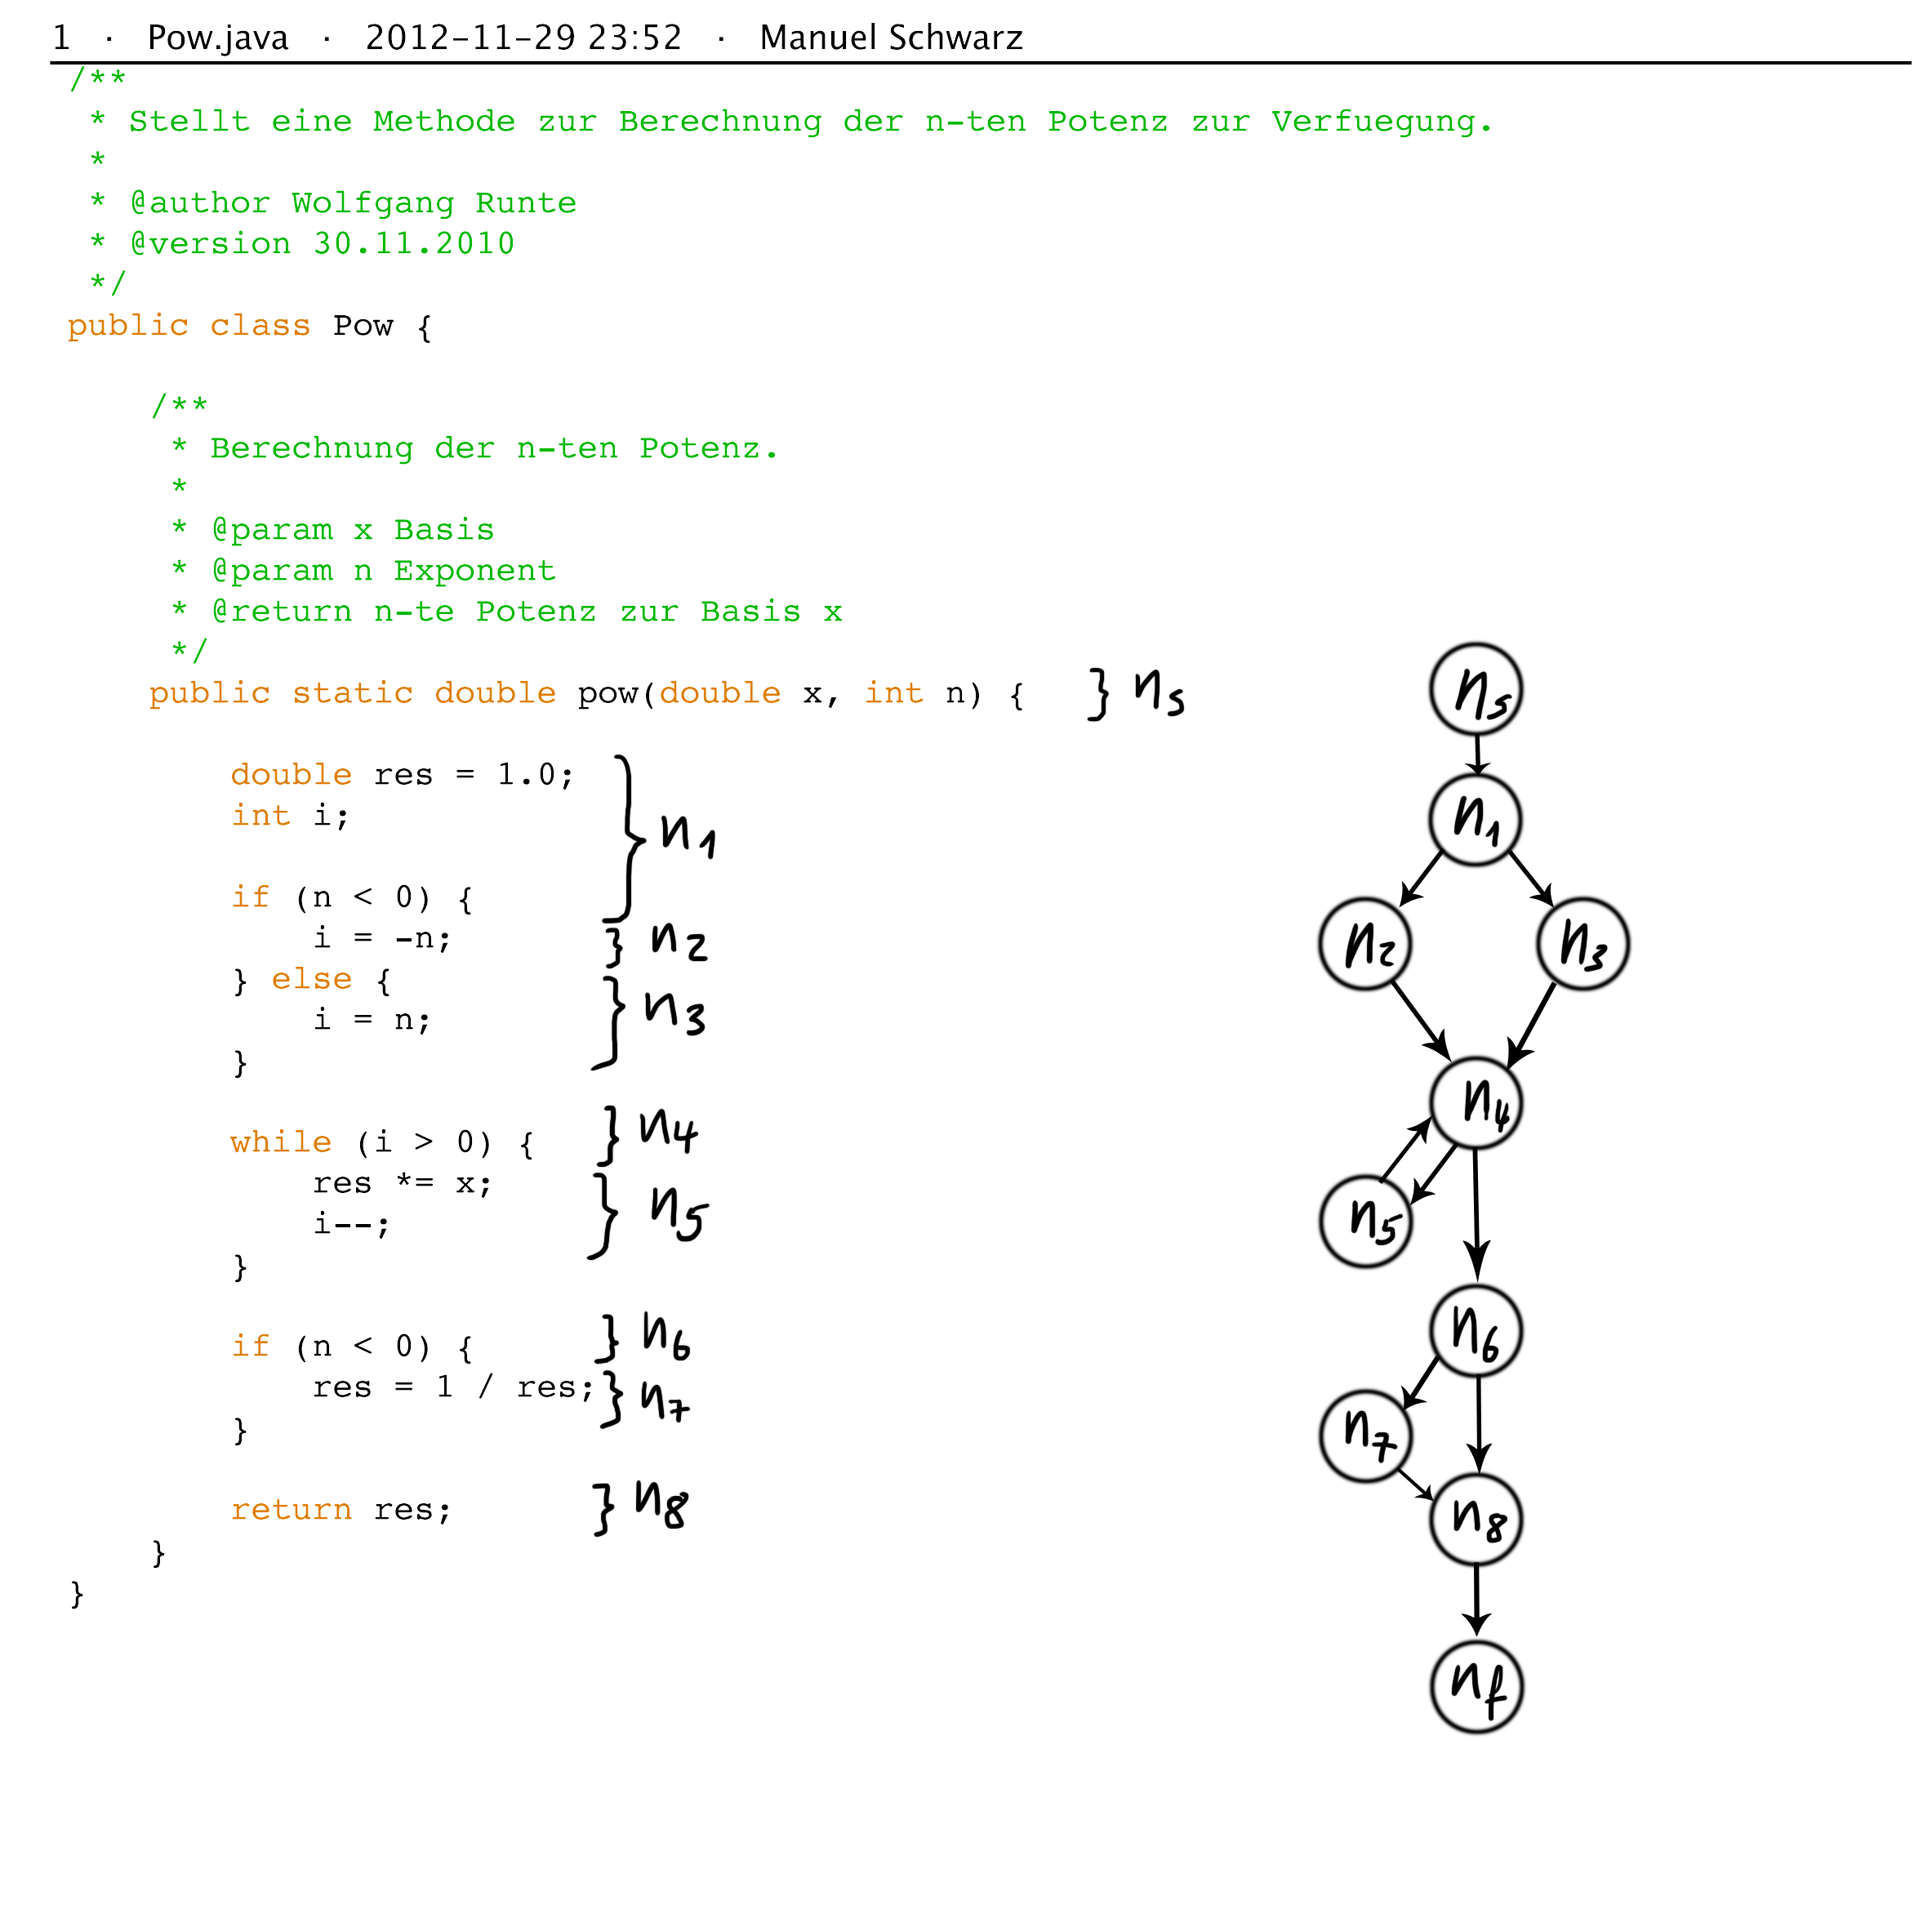
\includegraphics[width=\columnwidth]{Pow.png}

  \subsection*{(b) zyklomatische Komplexit�t}
  Die allgemeine Formel f�r die zyklomatische Komplexit�t eines Graphen $G$ lautet
  \begin{equation}
      Z(G) = e - n + 2
  \end{equation}
  Dabei beschreibt $e$ die Anzahl der Kanten und $n$ die Anzahl der Knoten von $G$.
  In unserem Fall gilt folglich:
  \begin{align*}
    Z(G) &= 12 - 10 + 2\\
    Z(G) &= 4
  \end{align*}


  \subsection*{(c) Bedeutung von $Z(G)$}
  Die Zahl sagt im allgemeinen etwas �ber die Komplexit�t der betrachteten
  Funktion aus, indem die Zahl bin�rer Verzweigungen gez�hlt wird. Weiterhin
  liefert sie direkt die Anzahl der maximal n�tigen Testf�lle und der
  Elementarpfade, da sie gleich der maximalen Anzahl linear unabh�ngiger
  gerichteter Zyklen entspricht.

  \subsection*{(d) Elementarpfade}
  \begin{tabular}{|c|c|c|c|c|c|c|c|c|c|c|c|c|}\hline
    Testf�lle / Kanten & 1 & 2 & 3 & 4 & 5 & 6 & 7 & 8 & 9 & 10 & 11 & 12\\\hline\hline
    I   &1&0&1&0&1&1&1&1&0&0&1&1\\\hline
    II  &1&1&0&1&0&1&1&1&1&1&0&1\\\hline
    III &1&0&1&0&1&0&0&1&0&0&1&1\\\hline
    IV  &1&1&0&1&0&0&0&1&0&0&1&1\\\hline
  \end{tabular}
  \\
  Testfall I (pos. Exp.): $n_s, n_1, n_3, n_4, n_5, n_4, n_6, n_8, n_f$\\
  Testfall II (neg. Exp.): $n_s, n_1, n_2, n_4, n_5, n_4, n_6, n_7, n_8, n_f$\\
  Testfall III (Exp. == 0): $n_s, n_1, n_3, n_4, n_6, n_8, n_f$\\
  Testfall IV: (unm�glich zu erzeugen):$n_s, n_1, n_2, n_4, n_6, n_8, n_f$\\

  \subsection*{(e) Linearkombination}
  Testfall I mit positivem Exponenten:
  \begin{equation*}
    (1 \cdot I) + (0 \cdot II) + (0 \cdot III) + (0 \cdot IV)
  \end{equation*}

  \subsection*{(f) Testf�lle}
  \begin{itemize}
    \item Testfall I: $x = 2$, $n = 2$
    \item Testfall II: $x = 2$, $n = -2$
    \item Testfall III: $x = 2$, $n = 0$
    \item Testfall IV: L�sst sich nicht erzeugen, da die Verzweigungen Abh�ngigkeiten untereinander haben,
          die im Widerspruch zu diesem Pfad stehen.
  \end{itemize}
\end{document}
